\begin{anexosenv}
% \chapter{Comandos seriais da estação meteorológica \textit{Vantage Vue™}} \label{anex:anexo1}

% \begin{center}
% \scalefont{0.85}
% \begin{longtable}{ll}
% \caption{Comandos seriais suportados pela estação meteorológica \textit{Vantage Vue™}}\\
% \hline
% \multicolumn{1}{c}{\textbf{Instrução}} & \multicolumn{1}{c}{\textbf{Descrição}} \\ \hline
% \endfirsthead

% \multicolumn{2}{c}%
% {{\bfseries \tablename\ \thetable{} -- Continuação da página anterior}} \\

% \hline
% \multicolumn{1}{c}{\textbf{Instrução}} & \multicolumn{1}{c}{\textbf{Descrição}} \\ \hline
% \endhead

% \multicolumn{2}{r}{{Continua na próxima página}} \\
% \endfoot

% \endlastfoot

% \multicolumn{2}{c}{\cellcolor{gray!25}\textbf{Comandos de teste}}                                                   		 \\ \hline
% \textbf{TESTE}                            & Envia a \textit{string} "TEST\textbackslash n" de volta  \\ \hline
% \textbf{WRD}                        & Responde com o tipo de estação meteorológica \\ \hline
% \textbf{RXCHECK}                        & Responde com o diagnóstico do Console \\ \hline
% \textbf{RXTEST}                       & Muda a tela do console de \textit{"Receiving from"} para tela de dados atuais                                                        \\ \hline
% \textbf{VER}                           & Responde com a data do \textit{firmware}                                                             \\ \hline
% \textbf{RECEIVERS}                    & Responde com a lista das estações que o console "enxerga" \\ \hline
% \textbf{NVER}                       & Responde com a versão do \textit{firmware}                                                             \\ \hline
% \multicolumn{2}{c}{\cellcolor{gray!25}\textbf{Comandos de dados atuais}}                                             \\ \hline
% \textbf{LOOP}                     & Responde com a quantidade de pacotes especificada a cada 2s        \\ \hline
% \textbf{LPS}                & Responde a cada 2s com a quantidade de pacotes diferentes especificada          \\ \hline
% \textbf{HILOWS}                & Responde com todo os dados de \textit{high/low}                 \\ \hline
% \textbf{PUTRAIN}                      & Seta a quantidade anual de precipitação \\ \hline
% \textbf{PUTET}                 & Seta a quantidade anual de evapotranspiração        \\ \hline
% \multicolumn{2}{c}{\cellcolor{gray!25}\textbf{Comandos de \textit{download}}}                                     		 \\ \hline
% \textbf{DMP}                 & Faz o \textit{download} de todo o arquivo de memória \\ \hline
% \textbf{DMAFT}                   & Faz o \textit{download} de todo o arquivo de memória após a data especificada \\ \hline
% \multicolumn{2}{c}{\cellcolor{gray!25}\textbf{Comandos da EEPROM}}                                     		 \\ \hline
% \textbf{GETEE}                 & Lê toda a memória EEPROM \\ \hline
% \textbf{EEWR}                   & Escreve um \textit{byte} de dados à partir do endereço especificado                                   \\ \hline
% \textbf{EERD}                   & Lê a quantidade de dados especificada iniciando no endereço especificado                                   \\ \hline
% \textbf{EEBWR}                   & Escreve os dados na EEPROM                                    \\ \hline
% \textbf{EEBRD}                   & Lê os dados da EEPROM \\ \hline
% \multicolumn{2}{c}{\cellcolor{gray!25}\textbf{Comandos de calibração}}                                     		 \\ \hline
% \textbf{CALED}                 & Envia os dados da temperatura e umidade corrente para atribuir à calibração \\ \hline
% \textbf{CALFIX}                   & Atualiza o \textit{display} quando os números de calibração mudam\\ \hline
% \textbf{BAR}                   & Seta os valores da elevação e o \textit{offset} do barômetro quando a localização é alterada                                   \\ \hline
% \textbf{BARDATA}                   & Mostra os valores atuais da calibração do barômetro                                   \\ \hline \\
% \multicolumn{2}{c}{\cellcolor{gray!25}\textbf{Comandos de limpeza}}                                     		 \\ \hline
% \textbf{CLRLOG}                 & Limpa todo o arquivo de dados                                                       \\ \hline
% \textbf{CLRALM}                   & Limpa todos os limiares dos alarmes                                   \\ \hline
% \textbf{CLRCAL}                   & Limpa todos os \textit{offsets} da calibração da temperatura e da umidade \\ \hline
% \textbf{CLRGRA}                   & Limpa o gráfico do console \\ \hline
% \textbf{CLRVAR}                   & Limpa o valor da precipitação ou da evapotranspiração \\ \hline
% \textbf{CLRHIGHS}                   & Limpa todos os valores de pico diários, mensais ou anuais                                   \\ \hline
% \textbf{CLRLOWS}                   & Limpa todos os valores de mínimos diários, mensais ou anuais \\ \hline
% \textbf{CLRBITS}                   & Limpa os \textit{bits} de alarme ativos                                  \\ \hline
% \textbf{CLRDATA}                   & Limpa todos os dados atuais                                   \\ \hline
% \multicolumn{2}{c}{\cellcolor{gray!25}\textbf{Comandos de configuração}}                                     		 \\ \hline
% \textbf{BAUD}                 & Atribui o valor do \textit{baudrate} do console                                                       \\ \hline
% \textbf{SETTIME}                   & Define a data e a hora do console                                   \\ \hline
% \textbf{GAIN}                   & Define o ganho do receptor de rádio                                   \\ \hline
% \textbf{GETTIME}                   & Retorna a hora e a data atual do console                                   \\ \hline
% \textbf{SETPER}                   & Define o intervalo de arquivamento                                   \\ \hline
% \textbf{STOP}                   & Desabilita a criação dos registros                                   \\ \hline
% \textbf{START}                   & Habilita a criação dos arquivos \\ \hline
% \textbf{NEWSETUP}                   & Reinicia o console após alguma configuração nova                                  \\ \hline
% \textbf{LAMPS}                   & Liga ou desliga as lâmpadas do console \\ \hline

% %\label{tab:6}
% \end{longtable}
% \fonte{\citeonline{VSPDOC} (Traduzido).}
% \end{center}

\partanexos % inicia a parte de anexos

\chapter{Modelo do sistema em caixa preta} % título do anexo
\label{anex:anexo1}

% Insere todas as páginas do PDF
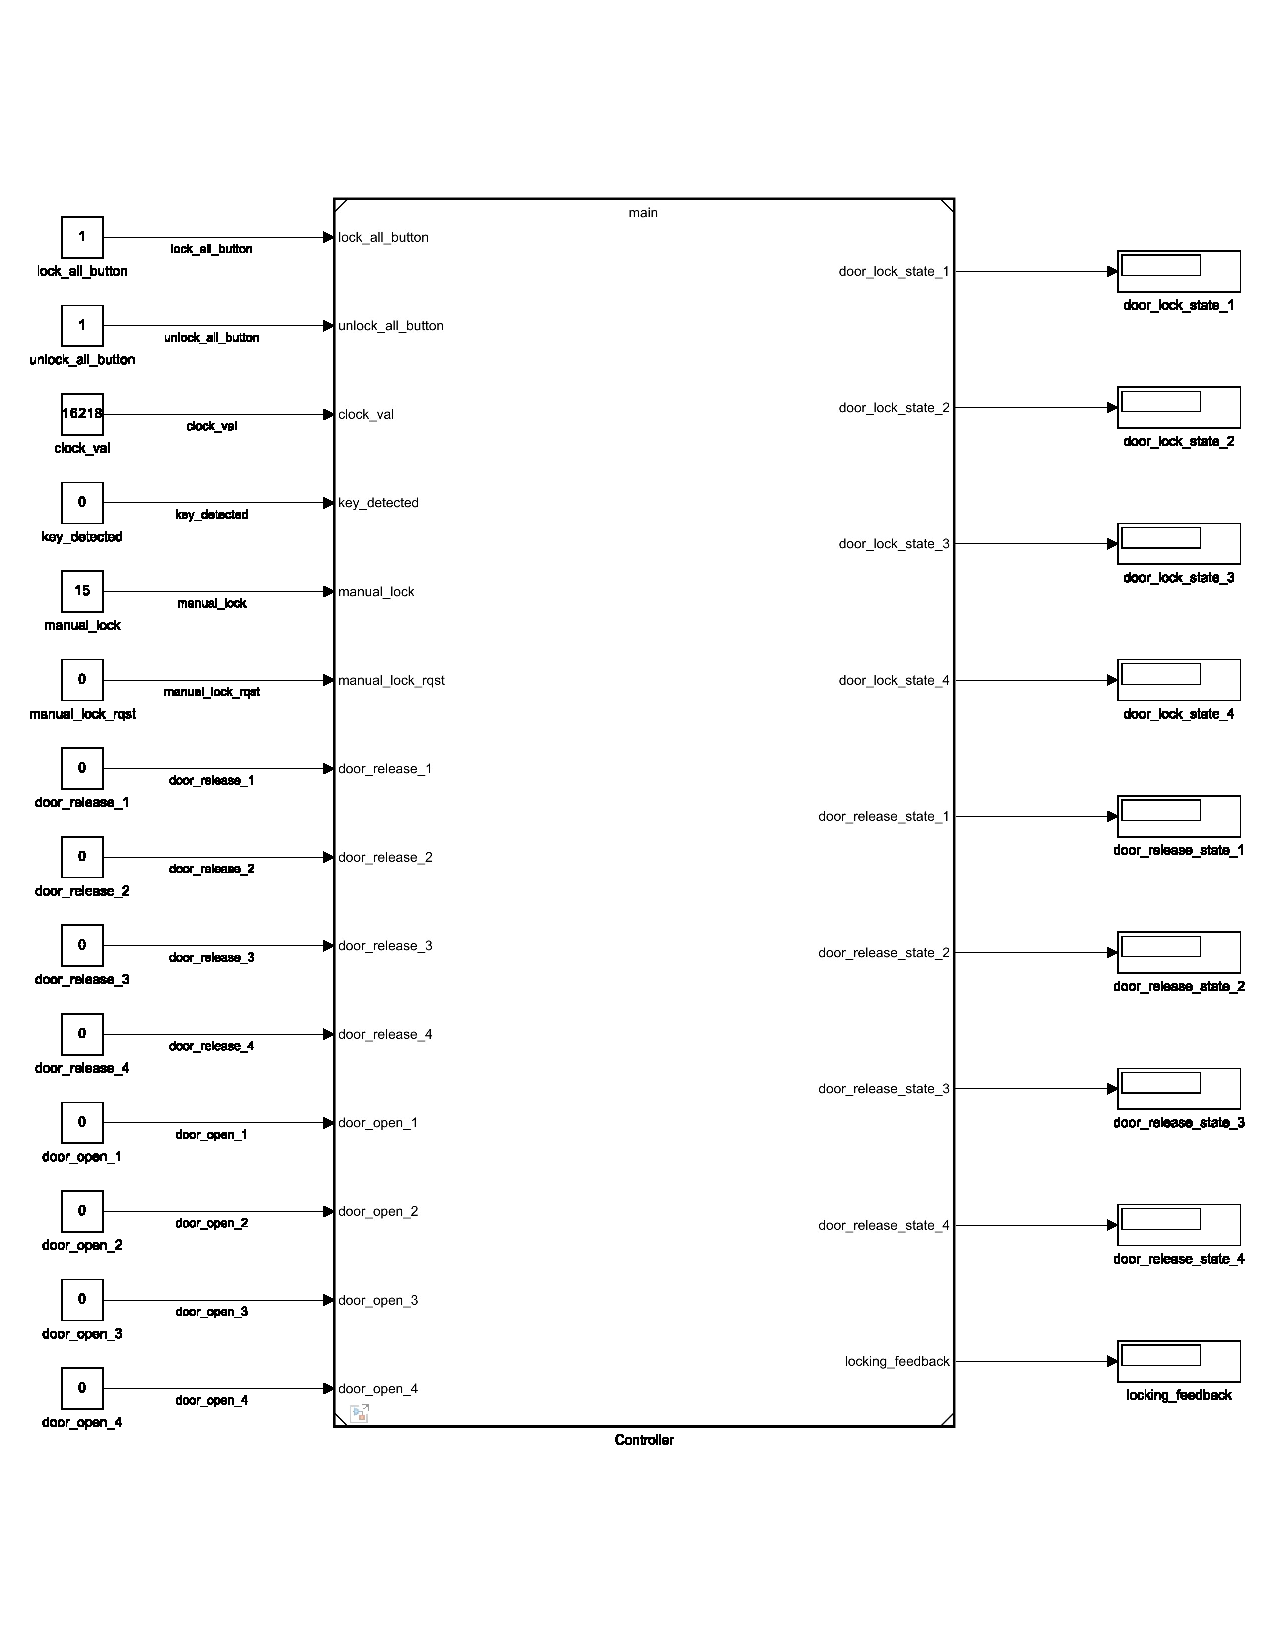
\includepdf[pages=-]{anexos/feature_model.pdf}

\end{anexosenv}
